
%% bare_conf.tex
%% V1.4b
%% 2015/08/26
%% by Michael Shell
%% See:
%% http://www.michaelshell.org/
%% for current contact information.
%%
%% This is a skeleton file demonstrating the use of IEEEtran.cls
%% (requires IEEEtran.cls version 1.8b or later) with an IEEE
%% conference paper.
%%
%% Support sites:
%% http://www.michaelshell.org/tex/ieeetran/
%% http://www.ctan.org/pkg/ieeetran
%% and
%% http://www.ieee.org/

%%*************************************************************************
%% Legal Notice:
%% This code is offered as-is without any warranty either expressed or
%% implied; without even the implied warranty of MERCHANTABILITY or
%% FITNESS FOR A PARTICULAR PURPOSE!
%% User assumes all risk.
%% In no event shall the IEEE or any contributor to this code be liable for
%% any damages or losses, including, but not limited to, incidental,
%% consequential, or any other damages, resulting from the use or misuse
%% of any information contained here.
%%
%% All comments are the opinions of their respective authors and are not
%% necessarily endorsed by the IEEE.
%%
%% This work is distributed under the LaTeX Project Public License (LPPL)
%% ( http://www.latex-project.org/ ) version 1.3, and may be freely used,
%% distributed and modified. A copy of the LPPL, version 1.3, is included
%% in the base LaTeX documentation of all distributions of LaTeX released
%% 2003/12/01 or later.
%% Retain all contribution notices and credits.
%% ** Modified files should be clearly indicated as such, including  **
%% ** renaming them and changing author support contact information. **
%%*************************************************************************


% *** Authors should verify (and, if needed, correct) their LaTeX system  ***
% *** with the testflow diagnostic prior to trusting their LaTeX platform ***
% *** with production work. The IEEE's font choices and paper sizes can   ***
% *** trigger bugs that do not appear when using other class files.       ***                          ***
% The testflow support page is at:
% http://www.michaelshell.org/tex/testflow/



\documentclass[conference]{IEEEtran}
% Some Computer Society conferences also require the compsoc mode option,
% but others use the standard conference format.
%
% If IEEEtran.cls has not been installed into the LaTeX system files,
% manually specify the path to it like:
% \documentclass[conference]{../sty/IEEEtran}





% Some very useful LaTeX packages include:
% (uncomment the ones you want to load)


% *** MISC UTILITY PACKAGES ***
%
%\usepackage{ifpdf}
% Heiko Oberdiek's ifpdf.sty is very useful if you need conditional
% compilation based on whether the output is pdf or dvi.
% usage:
% \ifpdf
%   % pdf code
% \else
%   % dvi code
% \fi
% The latest version of ifpdf.sty can be obtained from:
% http://www.ctan.org/pkg/ifpdf
% Also, note that IEEEtran.cls V1.7 and later provides a builtin
% \ifCLASSINFOpdf conditional that works the same way.
% When switching from latex to pdflatex and vice-versa, the compiler may
% have to be run twice to clear warning/error messages.






% *** CITATION PACKAGES ***
%
\usepackage{cite}
% cite.sty was written by Donald Arseneau
% V1.6 and later of IEEEtran pre-defines the format of the cite.sty package
% \cite{} output to follow that of the IEEE. Loading the cite package will
% result in citation numbers being automatically sorted and properly
% "compressed/ranged". e.g., [1], [9], [2], [7], [5], [6] without using
% cite.sty will become [1], [2], [5]--[7], [9] using cite.sty. cite.sty's
% \cite will automatically add leading space, if needed. Use cite.sty's
% noadjust option (cite.sty V3.8 and later) if you want to turn this off
% such as if a citation ever needs to be enclosed in parenthesis.
% cite.sty is already installed on most LaTeX systems. Be sure and use
% version 5.0 (2009-03-20) and later if using hyperref.sty.
% The latest version can be obtained at:
% http://www.ctan.org/pkg/cite
% The documentation is contained in the cite.sty file itself.






% *** GRAPHICS RELATED PACKAGES ***
%
\ifCLASSINFOpdf
   \usepackage[pdftex]{graphicx}
  % declare the path(s) where your graphic files are
   \graphicspath{{./pdf/}{./jpeg/}{./png/}}
  % and their extensions so you won't have to specify these with
  % every instance of \includegraphics
  % \DeclareGraphicsExtensions{.pdf,.jpeg,.png,.jpg}
\else
  % or other class option (dvipsone, dvipdf, if not using dvips). graphicx
  % will default to the driver specified in the system graphics.cfg if no
  % driver is specified.
  \usepackage[dvips]{graphicx}
  % declare the path(s) where your graphic files are
  % \graphicspath{{../eps/}}
  % and their extensions so you won't have to specify these with
  % every instance of \includegraphics
  % \DeclareGraphicsExtensions{.eps}
\fi
% graphicx was written by David Carlisle and Sebastian Rahtz. It is
% required if you want graphics, photos, etc. graphicx.sty is already
% installed on most LaTeX systems. The latest version and documentation
% can be obtained at:
% http://www.ctan.org/pkg/graphicx
% Another good source of documentation is "Using Imported Graphics in
% LaTeX2e" by Keith Reckdahl which can be found at:
% http://www.ctan.org/pkg/epslatex
%
% latex, and pdflatex in dvi mode, support graphics in encapsulated
% postscript (.eps) format. pdflatex in pdf mode supports graphics
% in .pdf, .jpeg, .png and .mps (metapost) formats. Users should ensure
% that all non-photo figures use a vector format (.eps, .pdf, .mps) and
% not a bitmapped formats (.jpeg, .png). The IEEE frowns on bitmapped formats
% which can result in "jaggedy"/blurry rendering of lines and letters as
% well as large increases in file sizes.
%
% You can find documentation about the pdfTeX application at:
% http://www.tug.org/applications/pdftex





% *** MATH PACKAGES ***
%
%\usepackage{amsmath}
% A popular package from the American Mathematical Society that provides
% many useful and powerful commands for dealing with mathematics.
%
% Note that the amsmath package sets \interdisplaylinepenalty to 10000
% thus preventing page breaks from occurring within multiline equations. Use:
%\interdisplaylinepenalty=2500
% after loading amsmath to restore such page breaks as IEEEtran.cls normally
% does. amsmath.sty is already installed on most LaTeX systems. The latest
% version and documentation can be obtained at:
% http://www.ctan.org/pkg/amsmath





% *** SPECIALIZED LIST PACKAGES ***
%
%\usepackage{algorithmic}
% algorithmic.sty was written by Peter Williams and Rogerio Brito.
% This package provides an algorithmic environment fo describing algorithms.
% You can use the algorithmic environment in-text or within a figure
% environment to provide for a floating algorithm. Do NOT use the algorithm
% floating environment provided by algorithm.sty (by the same authors) or
% algorithm2e.sty (by Christophe Fiorio) as the IEEE does not use dedicated
% algorithm float types and packages that provide these will not provide
% correct IEEE style captions. The latest version and documentation of
% algorithmic.sty can be obtained at:
% http://www.ctan.org/pkg/algorithms
% Also of interest may be the (relatively newer and more customizable)
% algorithmicx.sty package by Szasz Janos:
% http://www.ctan.org/pkg/algorithmicx




% *** ALIGNMENT PACKAGES ***
%
\usepackage{array}
% Frank Mittelbach's and David Carlisle's array.sty patches and improves
% the standard LaTeX2e array and tabular environments to provide better
% appearance and additional user controls. As the default LaTeX2e table
% generation code is lacking to the point of almost being broken with
% respect to the quality of the end results, all users are strongly
% advised to use an enhanced (at the very least that provided by array.sty)
% set of table tools. array.sty is already installed on most systems. The
% latest version and documentation can be obtained at:
% http://www.ctan.org/pkg/array


% IEEEtran contains the IEEEeqnarray family of commands that can be used to
% generate multiline equations as well as matrices, tables, etc., of high
% quality.



\usepackage{subcaption}
% *** SUBFIGURE PACKAGES ***
%\ifCLASSOPTIONcompsoc
%  \usepackage[caption=false,font=normalsize,labelfont=sf,textfont=sf]{subfig}
%\else
%  \usepackage[caption=false,font=footnotesize]{subfig}
%\fi
% subfig.sty, written by Steven Douglas Cochran, is the modern replacement
% for subfigure.sty, the latter of which is no longer maintained and is
% incompatible with some LaTeX packages including fixltx2e. However,
% subfig.sty requires and automatically loads Axel Sommerfeldt's caption.sty
% which will override IEEEtran.cls' handling of captions and this will result
% in non-IEEE style figure/table captions. To prevent this problem, be sure
% and invoke subfig.sty's "caption=false" package option (available since
% subfig.sty version 1.3, 2005/06/28) as this is will preserve IEEEtran.cls
% handling of captions.
% Note that the Computer Society format requires a larger sans serif font
% than the serif footnote size font used in traditional IEEE formatting
% and thus the need to invoke different subfig.sty package options depending
% on whether compsoc mode has been enabled.
%
% The latest version and documentation of subfig.sty can be obtained at:
% http://www.ctan.org/pkg/subfig




% *** FLOAT PACKAGES ***
%
\usepackage{fixltx2e}
% fixltx2e, the successor to the earlier fix2col.sty, was written by
% Frank Mittelbach and David Carlisle. This package corrects a few problems
% in the LaTeX2e kernel, the most notable of which is that in current
% LaTeX2e releases, the ordering of single and double column floats is not
% guaranteed to be preserved. Thus, an unpatched LaTeX2e can allow a
% single column figure to be placed prior to an earlier double column
% figure.
% Be aware that LaTeX2e kernels dated 2015 and later have fixltx2e.sty's
% corrections already built into the system in which case a warning will
% be issued if an attempt is made to load fixltx2e.sty as it is no longer
% needed.
% The latest version and documentation can be found at:
% http://www.ctan.org/pkg/fixltx2e


%\usepackage{stfloats}
% stfloats.sty was written by Sigitas Tolusis. This package gives LaTeX2e
% the ability to do double column floats at the bottom of the page as well
% as the top. (e.g., "\begin{figure*}[!b]" is not normally possible in
% LaTeX2e). It also provides a command:
%\fnbelowfloat
% to enable the placement of footnotes below bottom floats (the standard
% LaTeX2e kernel puts them above bottom floats). This is an invasive package
% which rewrites many portions of the LaTeX2e float routines. It may not work
% with other packages that modify the LaTeX2e float routines. The latest
% version and documentation can be obtained at:
% http://www.ctan.org/pkg/stfloats
% Do not use the stfloats baselinefloat ability as the IEEE does not allow
% \baselineskip to stretch. Authors submitting work to the IEEE should note
% that the IEEE rarely uses double column equations and that authors should try
% to avoid such use. Do not be tempted to use the cuted.sty or midfloat.sty
% packages (also by Sigitas Tolusis) as the IEEE does not format its papers in
% such ways.
% Do not attempt to use stfloats with fixltx2e as they are incompatible.
% Instead, use Morten Hogholm'a dblfloatfix which combines the features
% of both fixltx2e and stfloats:
%
% \usepackage{dblfloatfix}
% The latest version can be found at:
% http://www.ctan.org/pkg/dblfloatfix




% *** PDF, URL AND HYPERLINK PACKAGES ***
%
\usepackage{url}
\def\UrlBreaks{\do\/\do-\do+}
% url.sty was written by Donald Arseneau. It provides better support for
% handling and breaking URLs. url.sty is already installed on most LaTeX
% systems. The latest version and documentation can be obtained at:
% http://www.ctan.org/pkg/url
% Basically, \url{my_url_here}.




% *** Do not adjust lengths that control margins, column widths, etc. ***
% *** Do not use packages that alter fonts (such as pslatex).         ***
% There should be no need to do such things with IEEEtran.cls V1.6 and later.
% (Unless specifically asked to do so by the journal or conference you plan
% to submit to, of course. )


% correct bad hyphenation here
\hyphenation{N-A-D-I-R-N-Y-I-T}


\begin{document}
%
% paper title
% Titles are generally capitalized except for words such as a, an, and, as,
% at, but, by, for, in, nor, of, on, or, the, to and up, which are usually
% not capitalized unless they are the first or last word of the title.
% Linebreaks \\ can be used within to get better formatting as desired.
% Do not put math or special symbols in the title.
\title{Network Aware Defenses for Intrusion Recognition and Response (N.A.D.I.R.)}


% author names and affiliations
% use a multiple column layout for up to three different
% affiliations

%\author{\IEEEauthorblockN{Jonathan Voris}
%\IEEEauthorblockA{
%Email: jvoris@nyit.edu\\
%New York Institute of Technology\\
%New York, NY 10023\\}
%\and
%\IEEEauthorblockN{Yash Patel}
%\IEEEauthorblockA{
%Email: ypatel20@nyit.edu\\
%New York Institute of Technology\\
%New York, NY 10023\\}
%\and
%\IEEEauthorblockN{Nont Assawakomenkool}
%\IEEEauthorblockA{
%Email: nassawak@nyit.edu\\
%New York Institute of Technology\\
%New York, NY 10023\\}
%}

%Yash Author Custom
%
\author{\IEEEauthorblockN{Nont Assawakomenkool, Yash Patel, Jonathan Voris}
\IEEEauthorblockA{
$\left\{
nassawak@nyit.edu, ypatel20@nyit.edu, jvoris@nyit.edu
\right\}$\\
New York Institute of Technology\\
New York, NY 10023\\}
}

% conference papers do not typically use \thanks and this command
% is locked out in conference mode. If really needed, such as for
% the acknowledgment of grants, issue a \IEEEoverridecommandlockouts
% after \documentclass

% for over three affiliations, or if they all won't fit within the width
% of the page, use this alternative format:
%
%\author{\IEEEauthorblockN{Michael Shell\IEEEauthorrefmark{1},
%Homer Simpson\IEEEauthorrefmark{2},
%James Kirk\IEEEauthorrefmark{3},
%Montgomery Scott\IEEEauthorrefmark{3} and
%Eldon Tyrell\IEEEauthorrefmark{4}}
%\IEEEauthorblockA{\IEEEauthorrefmark{1}School of Electrical and Computer Engineering\\
%Georgia Institute of Technology,
%Atlanta, Georgia 30332--0250\\ Email: see http://www.michaelshell.org/contact.html}
%\IEEEauthorblockA{\IEEEauthorrefmark{2}Twentieth Century Fox, Springfield, USA\\
%Email: homer@thesimpsons.com}
%\IEEEauthorblockA{\IEEEauthorrefmark{3}Starfleet Academy, San Francisco, California 96678-2391\\
%Telephone: (800) 555--1212, Fax: (888) 555--1212}
%\IEEEauthorblockA{\IEEEauthorrefmark{4}Tyrell Inc., 123 Replicant Street, Los Angeles, California 90210--4321}}




% use for special paper notices
%\IEEEspecialpapernotice{(Invited Paper)}




% make the title area
\maketitle

% As a general rule, do not put math, special symbols or citations
% in the abstract
\begin{abstract}

It has become increasingly difficult to monitor computer networks as they have grown in scale and complexity. This lack of awareness makes responding to, or even recognizing, attacks a challenge. As a result, organizations' reactions to attacks are delayed, typically leaving them to address the situation long after an incident has taken place. The central idea behind this research is to provide earlier notification of potential network attacks by using deceptive network service information  as bait. These ''decoy'' or ''honey-services'' will indicate system weak points which do not exist when suspicious network circumstances are detected. That is, although up-to-date versions of the programs will be running on the system at all times, software versions with vulnerabilities will be advertised when a potential attack or reconnaissance effort is detected. Attacks against these services will be unsuccessful because the server running our system is not actually running the vulnerable services. By providing fake vulnerable points, our system is capable of collecting information about attacks earlier in the reconnaissance phase, potentially catching adversaries in the act without exposing any actual system weaknesses. Our solution effectively transforms any legitimate server into a ``honeypot'' without the added overhead of setting up and maintaining a set of fake network infrastructure.

\end{abstract}
% no keywords




% For peer review papers, you can put extra information on the cover
% page as needed:
% \ifCLASSOPTIONpeerreview
% \begin{center} \bfseries EDICS Category: 3-BBND \end{center}
% \fi
%
% For peerreview papers, this IEEEtran command inserts a page break and
% creates the second title. It will be ignored for other modes.
\IEEEpeerreviewmaketitle

\section{Introduction}
\label{introduction}

%Some do for fun, some do for money, some are insider attackers, and some are outsider adversaries.

Computer networks have become increasingly important components of people's everyday lives, and this trend seems poised to continue in the future. With this increased pervasiveness of networked systems
comes a commensurate increase in the number of people who attempt to break into them. Though a great deal of research effort has gone into preventing the exploitation of software vulnerabilities in order to
gain illicit remote access to computer systems, relatively little attention has been paid to interfering with attacks earlier in the attack life cycle, such as during the initial information gathering
stage. It has become increasingly difficult to monitor computer networks as they have grown in scale and complexity. This lack of awareness makes responding to, or even recognizing, attacks a challenge. As
a result, organizations' reactions to attacks are delayed, typically leaving them to address the situation long after an incident has taken place.

This work introduces the idea of creating a tool by utilizing existing network infrastructure features in order to provide Network Aware Defenses for Intrusion Recognition and Response (NADIR). The central
idea behind this research is to provide earlier notification of potential network attacks by using deceptive network service information  as bait. These ''decoy'' or ''honey-services'' will indicate system
weak points which do not exist when suspicious network circumstances are detected. That is, although up-to-date versions of the programs will be running on the system at all times, software versions with
vulnerabilities will be advertised when a potential attack or reconnaissance effort is detected. Attacks against these services will be unsuccessful because the server running our system is not actually
running the vulnerable services.

By providing fake vulnerable points, our system is capable of collecting information about attacks earlier in the reconnaissance phase, potentially catching adversaries in the act without exposing any
actual system weaknesses. Our solution effectively transforms any legitimate server into a ``honeypot'' without the added overhead of setting up and maintaining a set of fake network infrastructure.

In order to analyze network traffic to gain an understanding of contexts in which decoy service information should be deployed, we use a decision tree machine learning algorithm. Our system uses the Weka
machine learning toolkit \cite{misc:weka} to analyze, classify, and understand the structure of network traffic in order to infer when conditions are safe to reveal legitimate service details and when such
details should be masked with deceptive content.

%So that, we can move to the next step which is detecting and responding by using Snort \cite{roesch1999snort} in inline mode.

\begin{figure}[h!]
	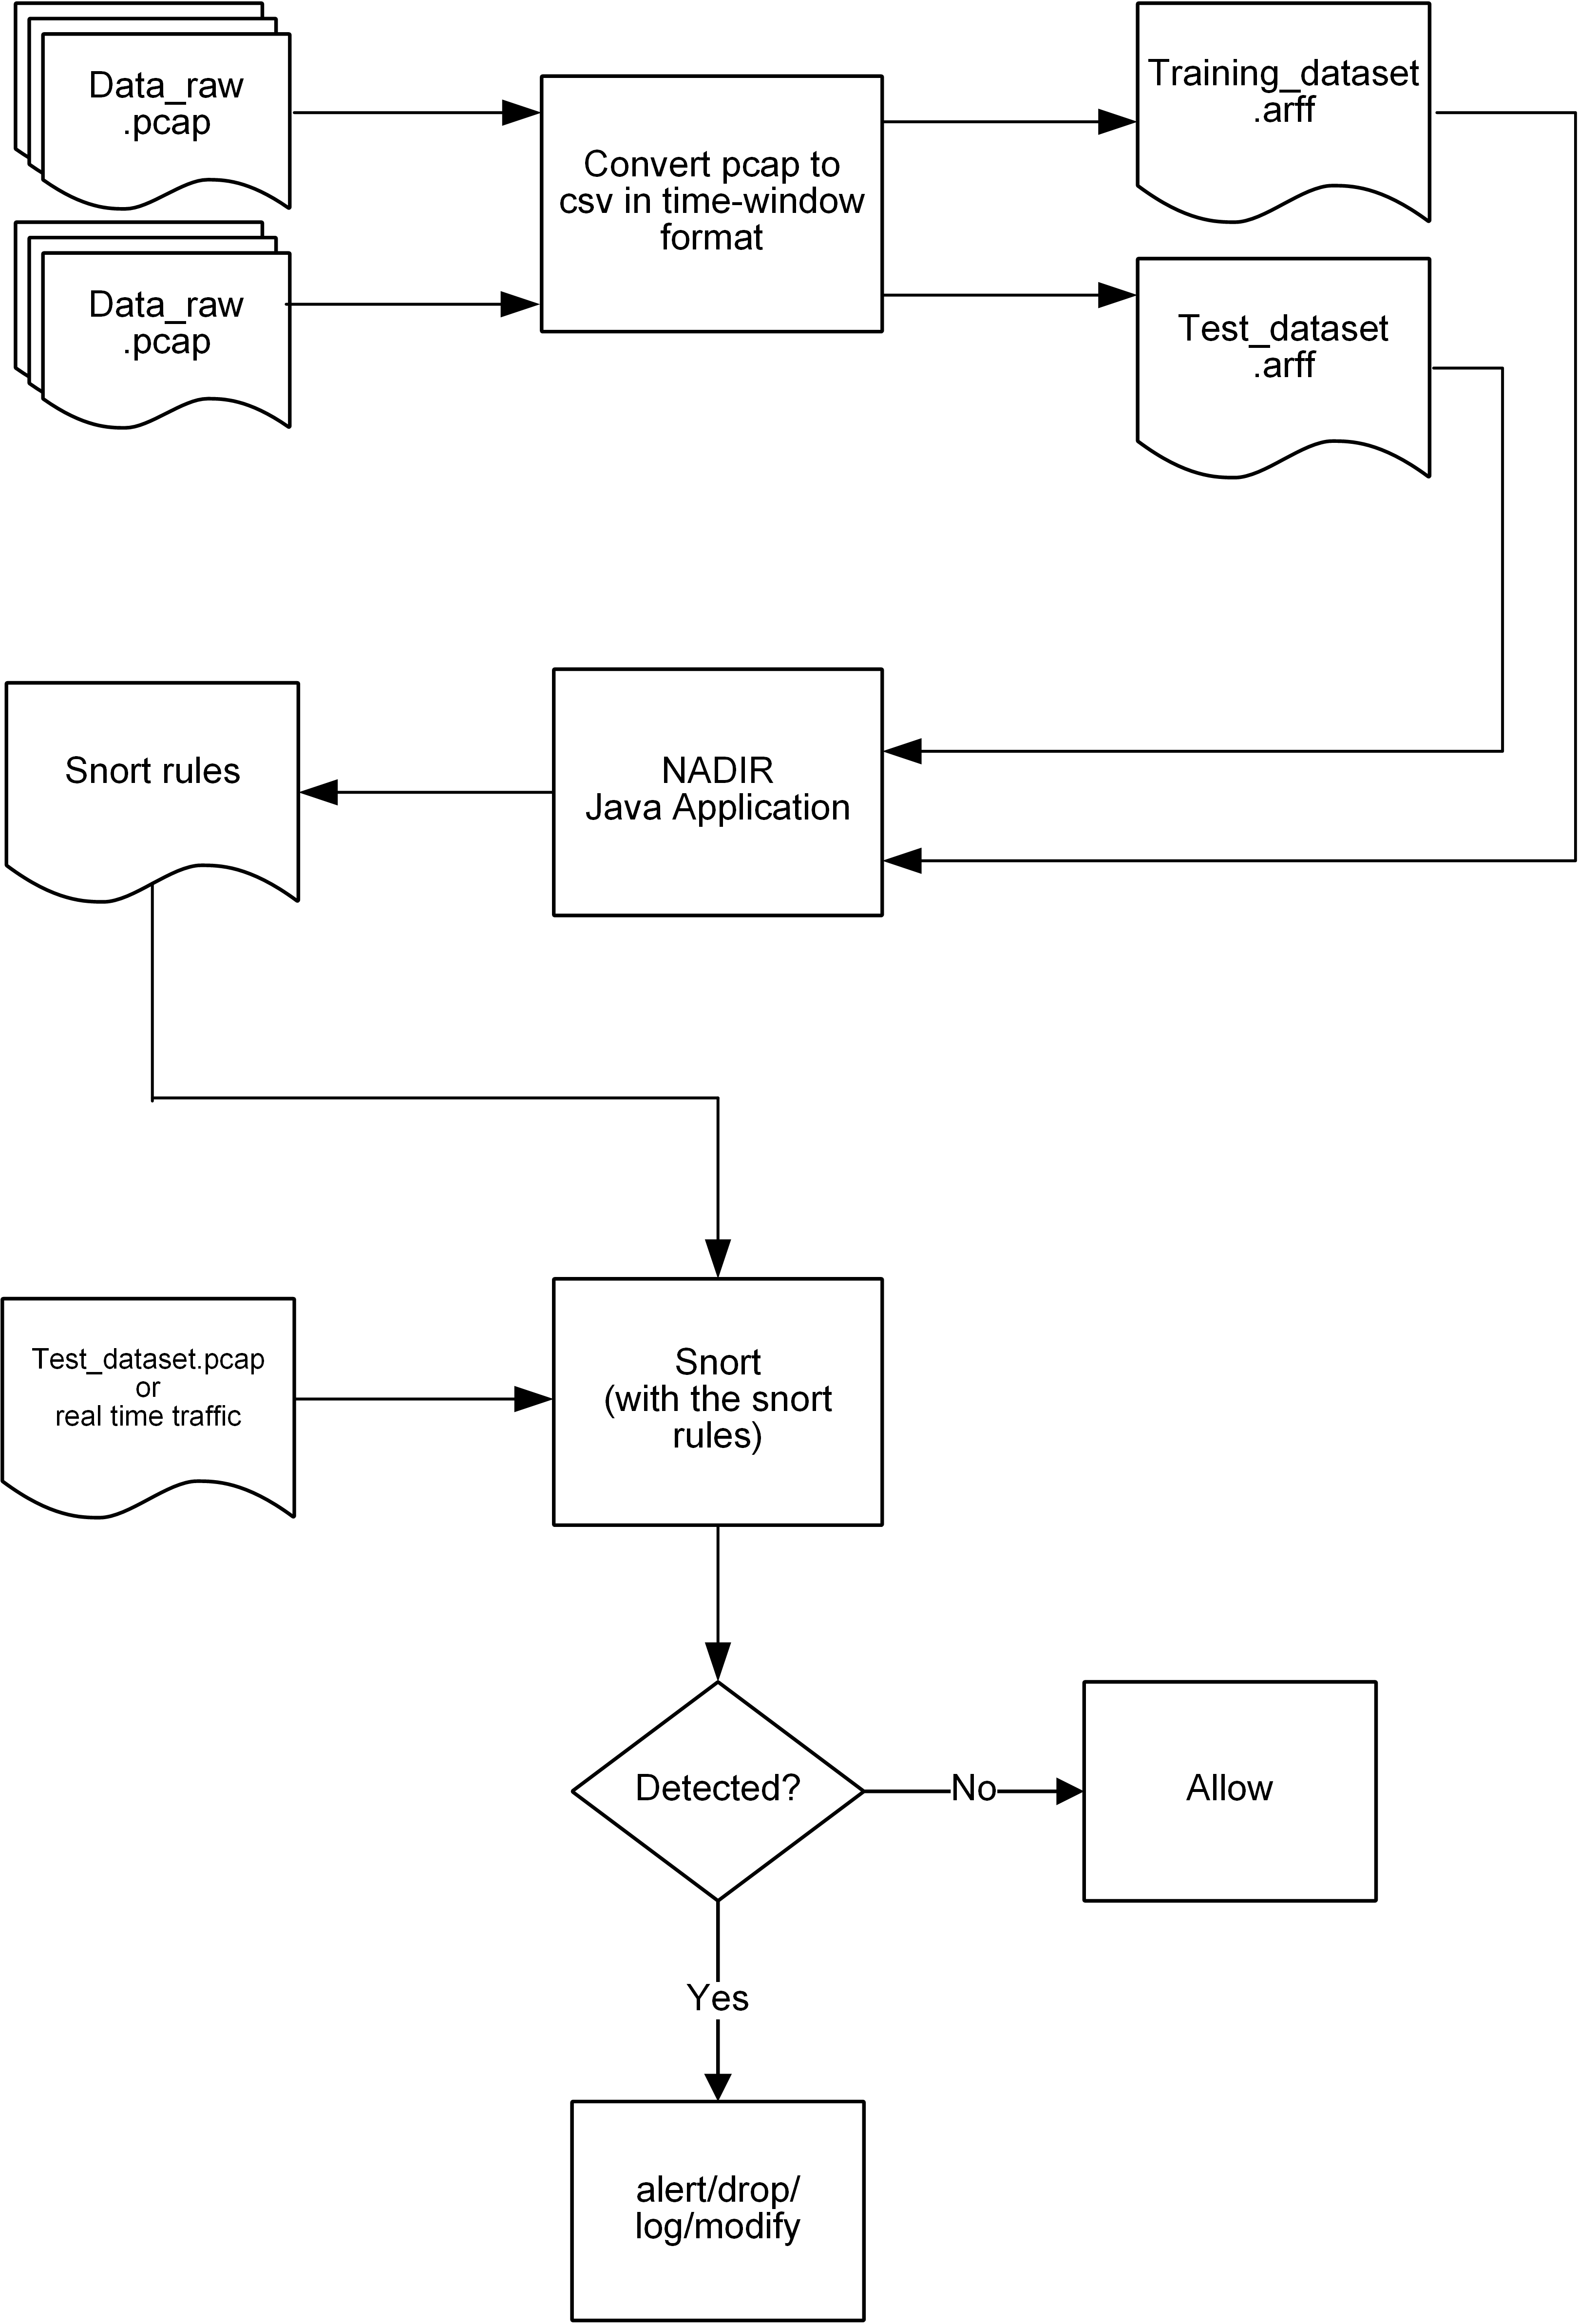
\includegraphics[width=\linewidth]{NADIR-processing_new_no_background.png}
	\caption{Over-all processing of NADIR System}
	\label{fig:overall}
\end{figure}

The overall workflow of our proposed system is shown as Figure \ref{fig:overall}. Our machine learning based technique is capable of classifying network traffic according to normal and abnormal patterns,
but several steps are required to process collected data prior to applying the classification algorithm. Firstly, we use an Intrusion Detection System (IDS) to collect network traffic data. In order to test
our system, we constructed a dataset comprised of the legitimate traffic observed by a test server on our university network as well as malicious traffic in the form of attacks we launched at known times to
provide ground truth.

Next, the collected network traffic data is converted into a Attribute-Relation File Format (ARFF) file for further processing. Subsequently, the NADIR system takes the network traffic data as input to
produces IDS rules based on what traffic was found to be indicative of an attack. Although any machine learning algorithm could potentially be used, we employed a decision tree classification algorithm to
produce IDS rules from the selected features automatically \cite{NetData2ARFF}. Finally, these rules are used to trigger our deception service description mitigation technique when unusual network
circumstances are detected.

The rest of the paper is organized as follows. Section \ref{related} discusses pertinent past research. Next, we present our threat model in Section \ref{threat_model}. The experiments we performed with our
system are presented in Section \ref{experiment} and their results are provided in \ref{results}. Finally, we conclude the paper in Section \ref{conclusion}.




\section{Related Work}
\label{related}

Network intrusion detection is a well-studied field, having been the focus of research for over two decades \cite{roesch1999snort, wang2004anomalous}. Approaches to intrusion detection can
typically be classified as rule-based, which are efficient but vulnerable to previously unobserved ``zero-day'' attacks, and anomaly based, which are capable of detecting novel attacks, but can be slow to
train and may incur high error rates. For example, a recent approach applied a neural network to classify traffic into normal and abnormal clusters \cite{NeuralNetBase}. Other approaches to learning for 
anomaly-based intrusion detection include Naive Bayes, Nearest neighbor, Decision Tree, and Support Vector Machines \cite{DMnIDS}. The most widely deployed IDS, Snort, is typically signature-based, but 
did support anomaly-based detection via the SPADE project \cite{SPADE}. Anomaly based intrusion detection approaches are orthogonal to this work, which instead focuses on leveraging network situational
awareness in order to adaptively respond to attacks.

As a result of the research activity in the area of IDS, several venerable network traffic datasets have been collected, including the DARPA \cite{DARPAdataset},  KDD-cup'99 \cite{tavallaee2009detailed},
and NSL-KDD \cite{lakhina2010feature} datasets. The goal of our research was not to improve upon the performance of prior approaches to anomaly detection, but rather to demonstrate how they could be
extended to create on-the-fly honeypots by combining them with our decoy service mitigation strategy. As such, we utilized these datasets as a foundation by deriving features from them which could be used
to detect network attacks which could be addressed with an adaptively service response. 

These datasets included network, system, and user-derived features \cite{AnalysisofNetfeatures}; we utilized the
available network level features which were available from these collections. More specifically, we chooses to focus our attention on three major attack categories: probe attacks and information collection
efforts, such as port scans, Denial-of-Service attacks, where a targeted network resource is exhausted, preventing legitimate access, and remote-to-local (R2L) attacks which exploit remote system
vulnerabilities in order to gain illicit system access. Although they have been used widely throughout the academic community, the aforementioned datasets are nearly two decades old, and as such are no
longer considered representative of current network traffic \cite{KDDharmful}; this motivated our collection of our own network intrusion testing dataset.

Another network defense option is to confuse and obstruct potential adversaries by providing deceptive information and decoy resources known as ``honeypots'' \cite{spitzner2003honeypots}. Honeypots, or 
decoy servers, are used to collect information on adversarial activity without risking any legitimate network assets. The Beeswarm project is an example of a honeypot deployment framework \cite{beeswarm}. 
A related defensive technology known as ``port hoping'' hides service information by rapidly altering the ports used by network services; only trusted clients aware of the anticipated pattern are able to 
gain access \cite{portHopping}. While honeypots and related techniques are powerful tools, they require substantial overhead to deploy and manage. Similarly, altering service characteristics such as port 
numbers constantly is a resource-intensive process. To address these shortcomings, our approach adaptively alters service characteristics only in response to detected threats.

%Snort IDS is one of active research area from last some decades and Snort has some features which can be changed and that useful to change IDS behavior and make it honeypot temporarily using snort rules
%\cite{signatureBaseIDSusingSnort}. Adaptive network response is most important part into the research our core goal for our research effort seeks to address this oversight by developing the novel 
%technique
%for detecting and responding to adversarial efforts to collect information about system they have targeted for attack \cite{aDeclarativeStateful}. We have not just focused on stop an attack but also catch
%attacker with sufficient evidence and take an action on machine to overcome performed attack. In contrast, the main idea behind our approach is to create a feedback mechanism whereby hosts, routers, and
%other devices can utilize current state information of network and alter network-facing properties to the attacker. By keep tracking network behavior and look at those anomalies and if the attack happens
%then dynamically change firewall rules and also change its state and also capture attack events is our core goal end of this research, By checking logs and detect and mitigate threat would be an advanced
%step which we could find in our application \cite{dynamicRuleCreation}. This how collected all important information and made background research more accurate and bidirectional in a way that we could 
%work
%on the actual experiment and its results and accuracy which we discussed in next part of this research paper.

%A related defensive technology known as ``port hoping'' hides service information by rapidly altering service ports 
%Threat detection and vulnerability patches are important though the easiest way to defend machine is to hide information or make the machine invisible into the network. \cite{spitzner2003honeypots}. 
%Honeypots, or decoy servers, are used to collect information on adversarial activity without . The machine placed where the inbound network traffic comes in through router, so the honeypot collects and %keeps track network
%traffic and its statistical behavior. It also has lots of research with threat detection used by honeypot service \cite{portHopping}. Honeypot the open source project for Ubuntu was the basic idea to %reply
%any request with fake packet information \cite{misc:honeypot}.

%We found snort had also suggested research on anomaly based detection by severity and anomaly score based
%preprocessor- SPADE which suspended for such reasons \cite{SPADE}. 

%Note that anomaly based intrusion detection approaches are orthogonal to this work, which instead focuses on leveraging network situational
%awareness in order to adaptively respond to attacks. By applying machine learning algorithm to classify threat from unknown data and pick those classifiers and used those features to get IDS rule sets to
%detect attacks in real-time. We have used decision tree classifier to get snort rule from selected features automatically from past research idea on snort rule generation mechanism by snort rule template
%using Association Rules Technique \cite{NetData2ARFF, misc:weka.jar}.

%Detecting threats against network by searching for anomalous traffic has been an active research area. We found
%various existing research idea and their suggested approaches include packet inspection, data mining techniques for feature selection, machine learning techniques such as Naive Bayes, Nearest neighbor,
%Decision tree and Support vector machines to detect intrusion over network \cite{DMnIDS}. We found snort had also suggested research on anomaly based detection by severity and anomaly score based
%preprocessor- SPADE which suspended for such reasons \cite{SPADE}. Note that anomaly based intrusion detection approaches are orthogonal to this work, which instead focuses on leveraging network
%situational awareness in order to adaptively respond to attacks. By applying machine learning algorithm to classify threat from unknown data and pick those classifiers and used those features to get IDS
%rule sets to detect attacks in real-time. We have used decision tree classifier to get snort rule from selected features automatically from past research idea on snort rule generation mechanism by snort
%rule template using Association Rules Technique \cite{NetData2ARFF, misc:weka.jar}.



%This section, we covered our background research related to our development. We began our research by observing and listing useful features for anomaly based intrusion detection used in previous %researches
%and as suggested we collected and listed features by looking at different dataset for intrusion detection. We have started our research by work on DARPA, NSL-KDD, KDD-cup'99 dataset and understand dataset
%methodology. They have included Network based, System based as well as User based features into the NSL-KDD, KDD-cup'99 dataset \cite{AnalysisofNetfeatures}. DARPA-pi introduces the dataset for network
%simulation and we found they collected unlabeled dataset which can be divided into clusters by normal or abnormal behavior of network \cite{DARPAdataset,NeuralNetBase}. Such as, we have focused on network
%threats only that includes ten different attacks and divided into three major types in our research. In which we covered Port Scanning (Probe) - gathering network information to bypass security, Denial of
%Service (Dos)-where some resource is swamped; causing DoS to legitimate users, Remote to local (R2L)-attacks that exploit remote system vulnerabilities to get access to a system\cite{R2L}.

%As KDD- cup'99 is really basic idea and it also has been long history in performance on anomaly based intrusion detection, but we realized it outdated and not much fit with our model, so finally We
%collected and built our own dataset for different network attacks with legitimate traffic. 






\section{Threat model}
\label{threat_model}

In our research, we assume that all conditions of attack are based on remote attacks. It means “no adversaries can get into a target server physically, but they can exploit the target server remotely. The attackers know nothing about the N.A.D.I.R. system so that they attack the target server with no suspect. The attackers use some tools for scanning the target server's running services to learn the information of those services and look for a vulnerable service(s). Once they know the vulnerable service(s) on the target server, they can use other tools to attack the target through that service(s) to down the service or to gain an access so they can do more business. Which this threat model, the N.A.D.I.R. system takes an action at the first place where the attackers scan the running services on the server. The N.A.D.I.R. system hides the true information of running services then sends the decoy services' information back to the attackers. Thus, we can detect and catch the attackers who attack the decoy services.


\section{Experiment}
\label{experiment}


\subsection{Network Setup and Launch Attack}

In this part of research, we cover introduction of our testing environment and also experimental setup of those machines. We have installed and configured three Virtual Machines - Victim, Attacker and Vulnerable. All virtual machines are run on the same individual server, but they are separate in logical. The traffic flow between each machines are shown in Figure \ref{fig:connectionModel}. In which victim's VM configured with snort, attacker's machine contains Metasploit tool-kit and we used existing vulnerable Ubuntu operating system for testing purposes and make it as our third machine - vulnerable \cite{misc:metasploitable}. We have deployed and tested ten different Metasploit attacks and we divided it into three types of attack including Port Scanning (Probe) - gathering network information to bypass security, Denial of Service (Dos) - where some resource is swamped; causing DoS to legitimate users, Remote to local (R2L) - attacks that exploit remote system vulnerabilities to get access to a system. After successfully tested we made all of them as automated handled by Metasploit script, which we used for development of attacker's system\cite{misc:metasploitScripts}.


\begin{figure}[h!]
	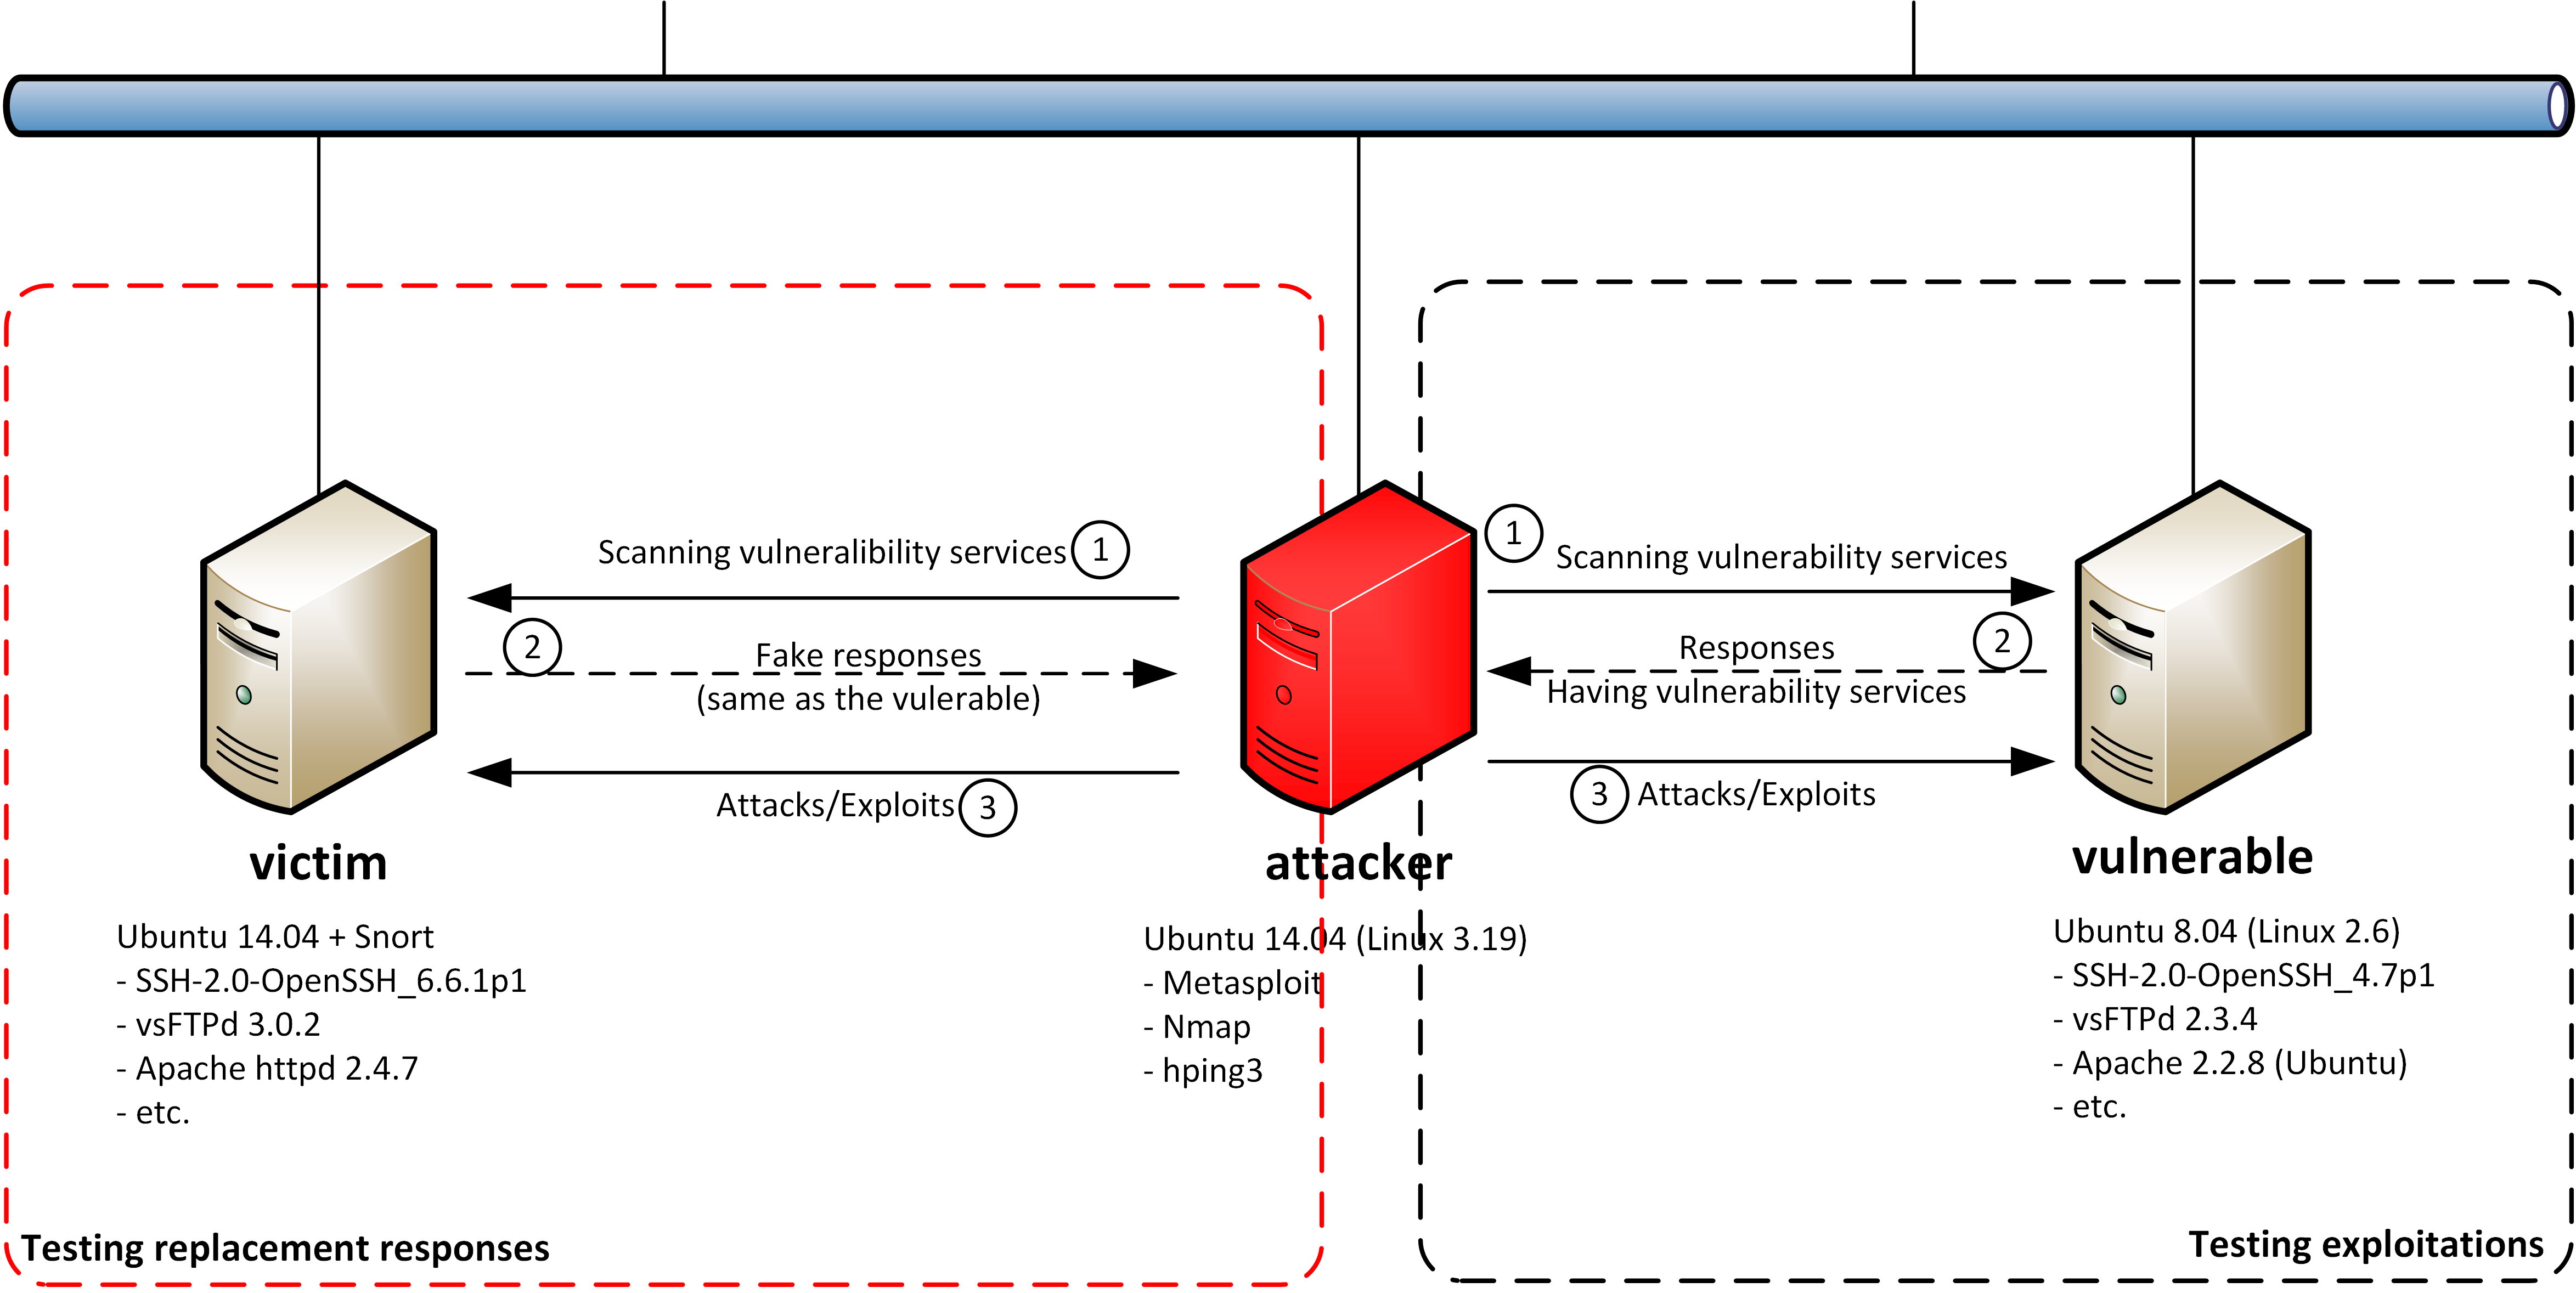
\includegraphics[width=\linewidth]{networkSecurityResearch_new_no_back.png}
	\caption{Logical connection model}
	\label{fig:connectionModel}
\end{figure}

\subsection{Dataset preparation}

%We started research to work on dataset preparation by taking existing dataset and run their suggested machine learning techniques using weka tool. And when we were %working on KDD- cup'99 dataset we found it was really outdated as it was to older and those number of features which they have focused on, it was not applicable with %our research because we focused on network threat as we were looking at network behavior and traffic for anomaly detection for intrusion detection %system\cite{anomaly-basedNID}. 

In this part of research to collect and extract dataset we started data modeling with existing different labeled datasets to understand the model of machine learning. Then we worked on existing datasets to extract usable features from it and we came up with the java parser script which can parse and extract entire data information from Pcap file and saved into Csv file. We put time-window size variable to extract and identify unique combinations of packet transmission. Parser can parse and split the entire Pcap information with respect to the time-window size. While researching on previous suggested approaches we tried to extract dataset by different time-windows size by changing its value by 10 seconds, 1 seconds, 7 seconds, and 5 seconds. We observe that 4 second time frame is more preferable in our network architecture as it generate more accurate result with weka. As this feature is flexible and it is depends on the nodes in our network. We collected and built our own datasets to test our model and accuracy of algorithms for anomaly detection of network attacks \cite{DMnIDS}. We launch each attack repeatedly and capture those Pcap and after merging those Pcap we extract that into Csv format using our own Csv-parser by 4 second time window size.

\begin{figure}[h!]
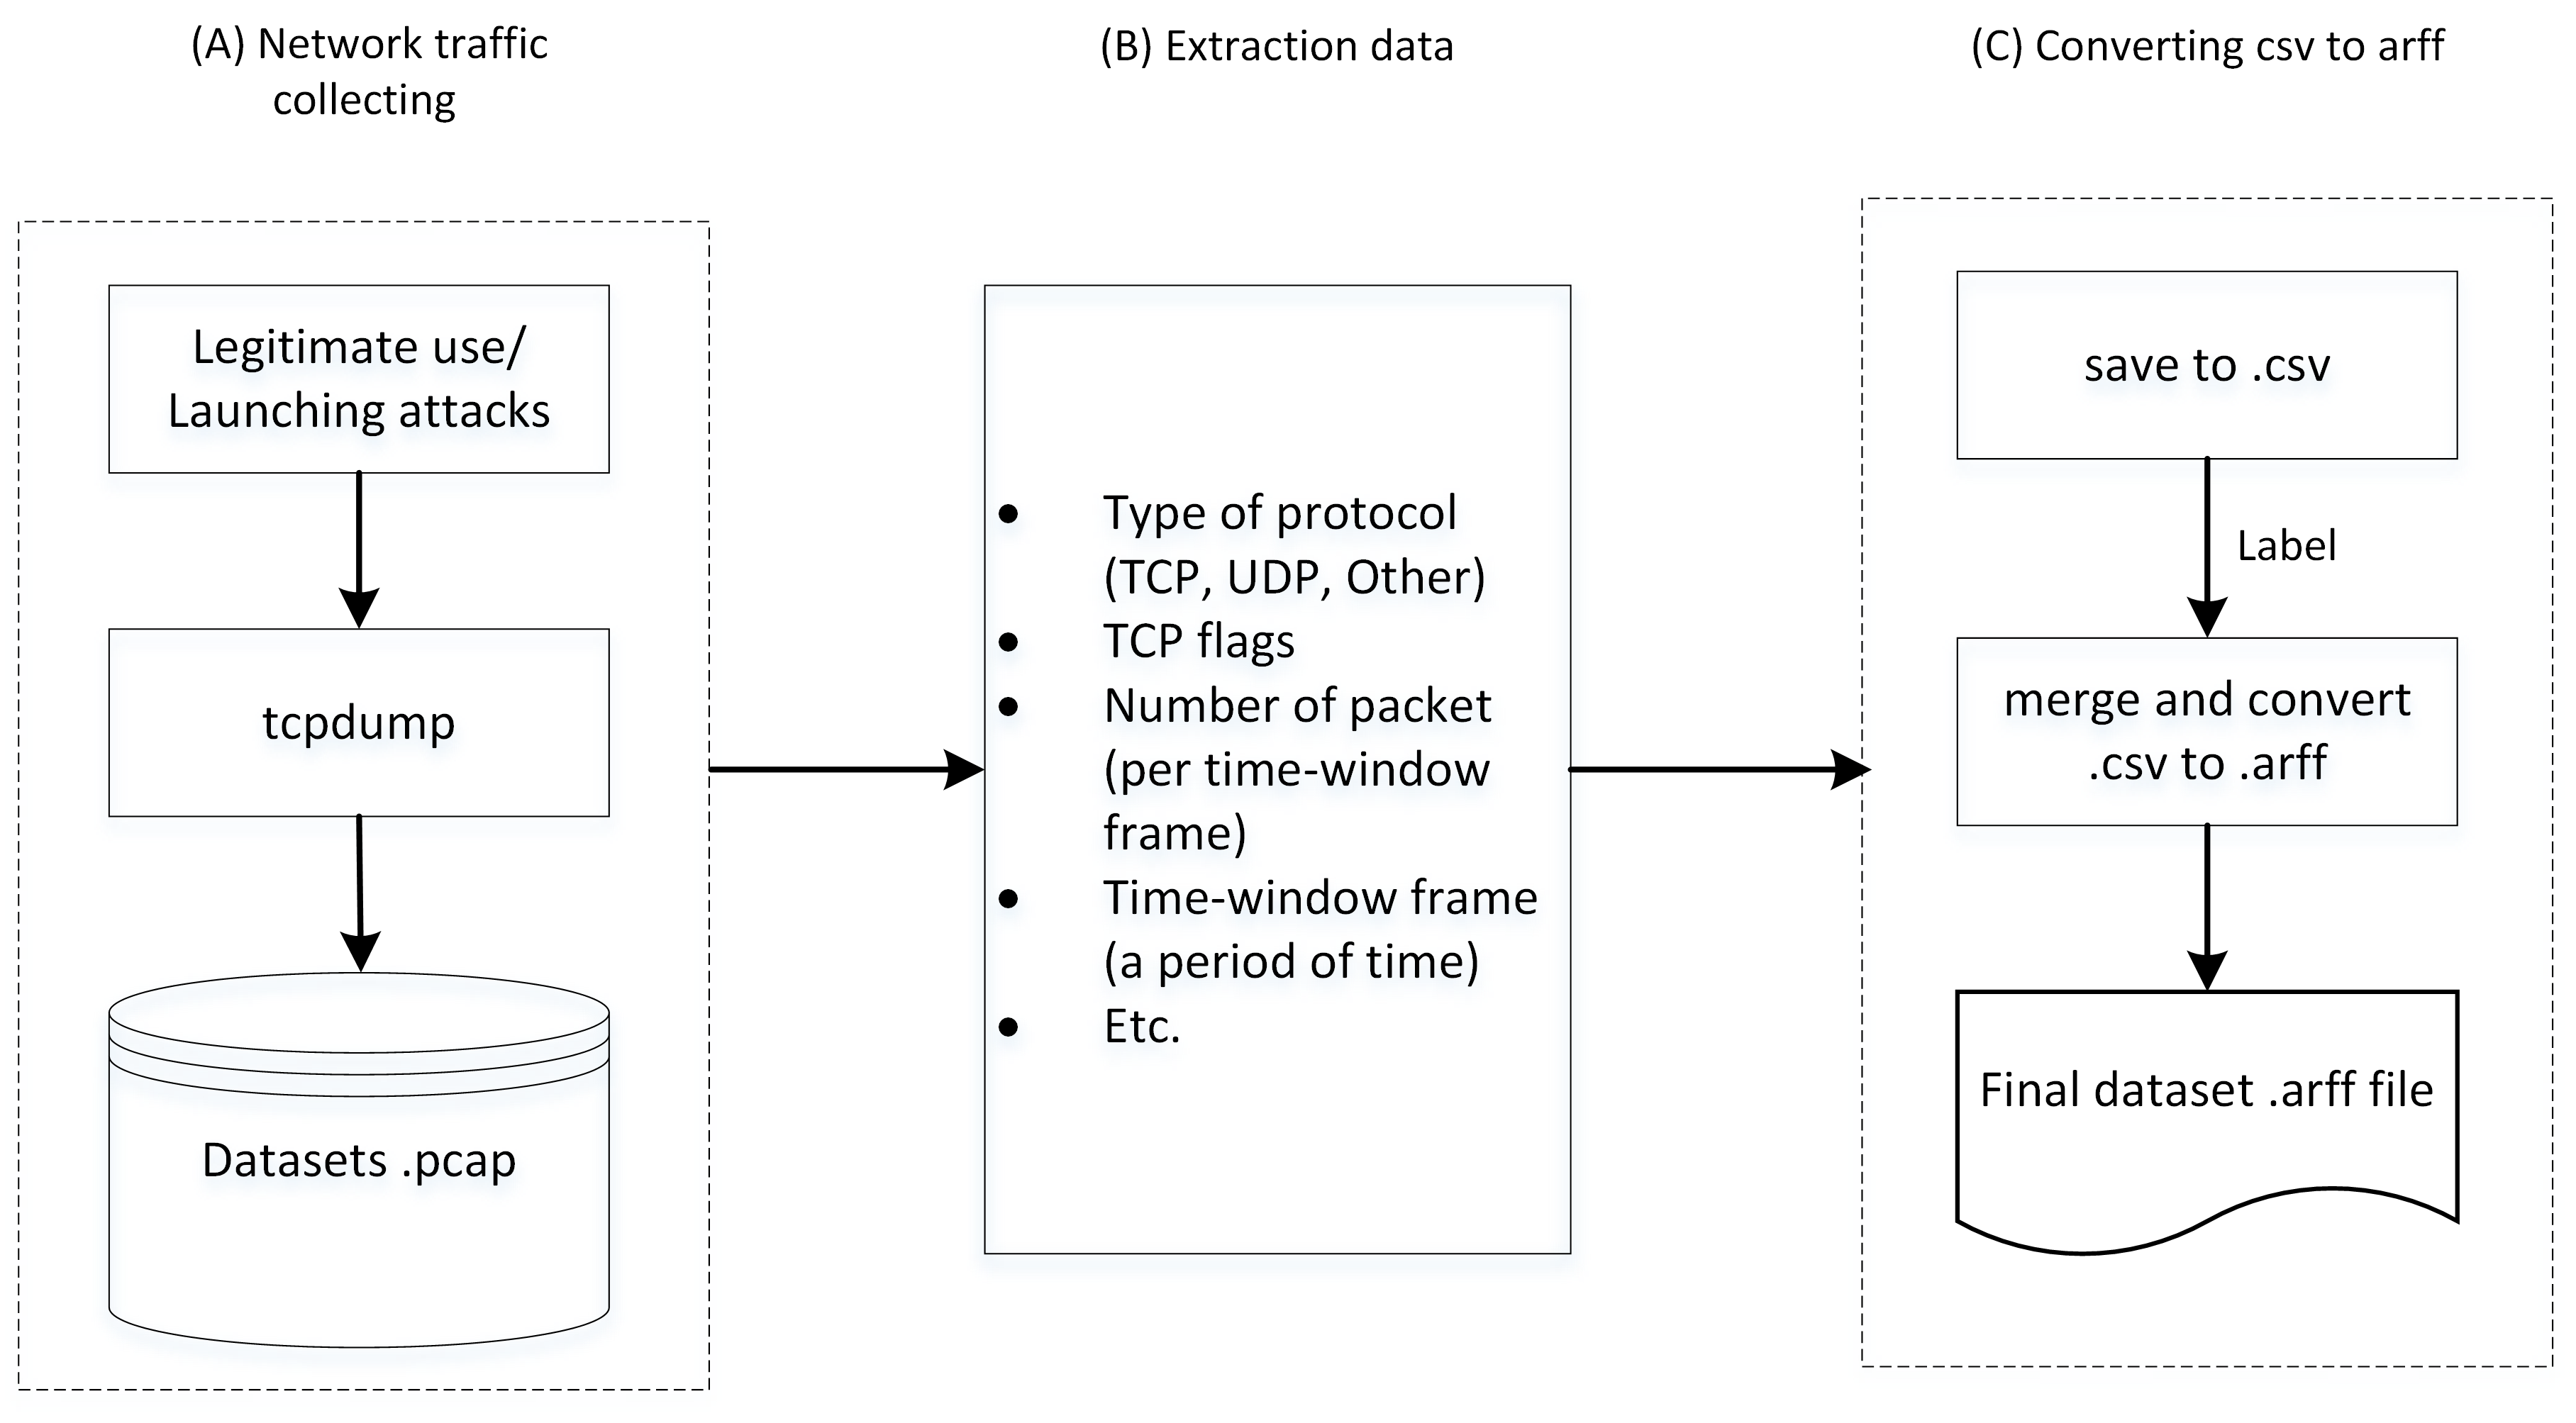
\includegraphics[width=\linewidth]{dataset_preparation_no_background.png}
\caption{Process of dataset preparation}
\label{fig:dataset_prepare}
\end{figure}

\noindent Each row into the final Csv represents a unique direction from source\_ip to destination\_ip for 4sec time window. List of features which we covered into dataset is shown in the Table \ref{table:features} and the dataset preparation process is shown as Figure \ref{fig:dataset_prepare}.

\begin{table}
\begin{center}
\begin{tabular}{|p{3.1cm}|p{4.9cm}|}
\hline
\multicolumn{1}{|c|}{\bfseries Name of Feature} & \multicolumn{1}{c|}{\bfseries Description}\\
\hline
TYPE\_PACKET & Which type of packet – tcp, udp and other into string\\
\hline
FIRST\_TIMESTAMP & Arriving timestamp when the first packet received into numeric\\
\hline
NO\_OF\_PACKETS & No of packets how much received into numeric\\
\hline
DEST\_IP & Destination IP into string\\
\hline
SOURCE\_IP & Source IP into string\\
\hline
TCP\_FIN & Sum of TCP FIN flags into numeric\\
\hline
TCP\_SYN & Sum of TCP SYN flags into numeric\\
\hline
TCP\_RST & Sum of TCP RST flags into numeric\\
\hline
TCP\_PSH & Sum of TCP PSH flags into numeric\\
\hline
TCP\_ACK & Sum of TCP ACK flags into numeric\\
\hline
TCP\_URG & Sum of TCP URG flags into numeric\\
\hline
TCP\_ECE & Sum of TCP ECE flags into numeric\\
\hline
TCP\_CWR & Sum of TCP CWR flags into numeric\\
\hline
ETHER\_TYPE\_AVG & Average of Ethernet type into numeric\\
\hline
WIRELEN\_AVG & Average of Ethernet Wirelen into numeric\\
\hline
IP\_OFFSET\_AVG & Average of IP Offset value into numeric\\
\hline
IP\_LENGTH\_AVG & Average of IP Length value into numeric\\
\hline
IP\_VER\_AVG & Average of IP Version value into numeric\\
\hline
IP\_HLEN\_AVG & Average of IP hlen value into numeric\\
\hline
IP\_TTL\_AVG & Average of IP ttl value into numeric\\
\hline
IP\_FLAG\_AVG & Average of IP flag value into numeric\\
\hline
IP\_TYPE\_AVG & Average of IP type value into numeric\\
\hline
TCP\_OFFSET\_AVG & Average of TCP Offset value into numeric\\
\hline
TCP\_LENGTH\_AVG & Average of TCP Length value into numeric\\
\hline
TCP\_HLEN\_AVG & Average of TCP hlen value into numeric\\
\hline
TCP\_RESERVE\_AVG & Average of TCP Reserve value into numeric\\
\hline
TCP\_WINDOW\_AVG & Average of TCP Window size value into numeric\\
\hline
TCP\_URGENT\_AVG & Average of TCP Urgent value into numeric\\
\hline
PAYLOAD\_OFFSET\_AVG & Average of Payload Offset value into numeric\\
\hline
PAYLOAD\_LENGTH\_AVG & Average of Payload Length value into numeric\\
\hline
ANOMALY\_SCORE & Class feature to label pattern (NORMAL/NMAP/DOS/R2L)\\
\hline
\end{tabular}
\end{center}
\caption{Table of feature extraction}
\label{table:features}
\end{table}

\noindent We added time window size parameter flexible that in future one can change this parameter for their use by observing network traffic. We launched each attacks from attacker's machine and we assume that all the packets which are coming from that attacker's machine as an attack and then we labeled our dataset manually attacks and normal and converted into arff file format for development. We ignore and remove SOURCE\_IP, DESTINATION\_IP, and FIRST\_TIMESTAMP because we observe it somehow classified pattern by taking those specific values. So after removed those features we are just looking at network behavioral features and extracting those to classify and generate snort rule dynamically for matched patterns.



\subsection{Data modeling and Machine learning}

Weka library is one of the famous open source library for data mining and machine learning \cite{misc:wekaTutorial}. It provides various algorithm and methods to work on any types of dataset to extract useful features which can applies to identify more accurately and our research Began with dataset preparation to build and train our model. We used ANOMALY\_SCORE class variable to predict a specific pattern for normal or attack into dataset. Decision tree is used where dataset has some predictor by which pattern can be classified into appropriate class. In our research we used J48 algorithm which is easy to convert into conditional algorithm for automatic snort rule generation \cite{misc:weka.jar}. We used weka.jar library to implement J48 decision tree java program. Conditional program generated through weka by taking labeled training dataset as an input. It uses program template in which we designed snort rule template with weka static method call which takes labeled/unlabeled testing dataset and generates snort rules by looking at matched attack patterns and its classified feature values..

We used J48 decision tree machine learning algorithm to train the model as well as snort rule generation by using that model \cite{NIDusingDT}. J48 decision tree classifier classify pattern by number of feature from our dataset which we than converted into snort rule using snort rule template. For example if model classified a specific attack pattern by tcp\_syn, no\_packets and type\_packet features than it will put those values of that specific features into snort rule template which we used into our Java application and as an output of that program we get snort rules.

%alert tcp \$EXTERNAL\_NET any -$>$ \$HOME\_NET any (msg: "[*] Attack-detected on S"; flags: S; flow: from\_client; threshold: type both, track by\_dst, count 182765, %seconds 4; sid: 3000001 ;)


\subsection{Snort configuration}

Intrusion Detection System (IDS) is a device which monitors packets on your network. IDS reports attack behaviors based on rules and signatures applied to the machine. IPS could achieve Real-time intercepting by leveraging in-line deployment in the network. It analyzes all network traffic passing through interface and takes actions to suspicious packets immediately\cite{misc:netfilter}.

We converted Snort IDS into INLINE QUEUE mode by using Iptables rule and Snort configurations. Now, it receives packets sent from the Net filter Queue with the help of the nfnetlink\_queue library, compares them with Snort signature rules and alert or drop if they match a rule, then finally sends them back to Net filter Queue where the Snort Inline tagged packets are dropped \cite{misc:netfilter}. An IPS (Intrusion Prevention System) where a packet matching a signature rule is blocked or modified.

In this case, the attacker will get the same information or fingerprints as the responses from the Vulnerable when the Attacker scans vulnerability services on the victim which are fake responses (replaced payload packets). For example, the attacker gets a fingerprint of version of SSH service from the Vulnerable as SSH-2.0-OpenSSH-4.7p1 and gets the same information, SSH-2.0-OpenSSH-4.7p1, from Victim as well even though the corrected information is SSH-2.0-OpenSSH-6.6.1p1.

%\begin{figure}[h!]
%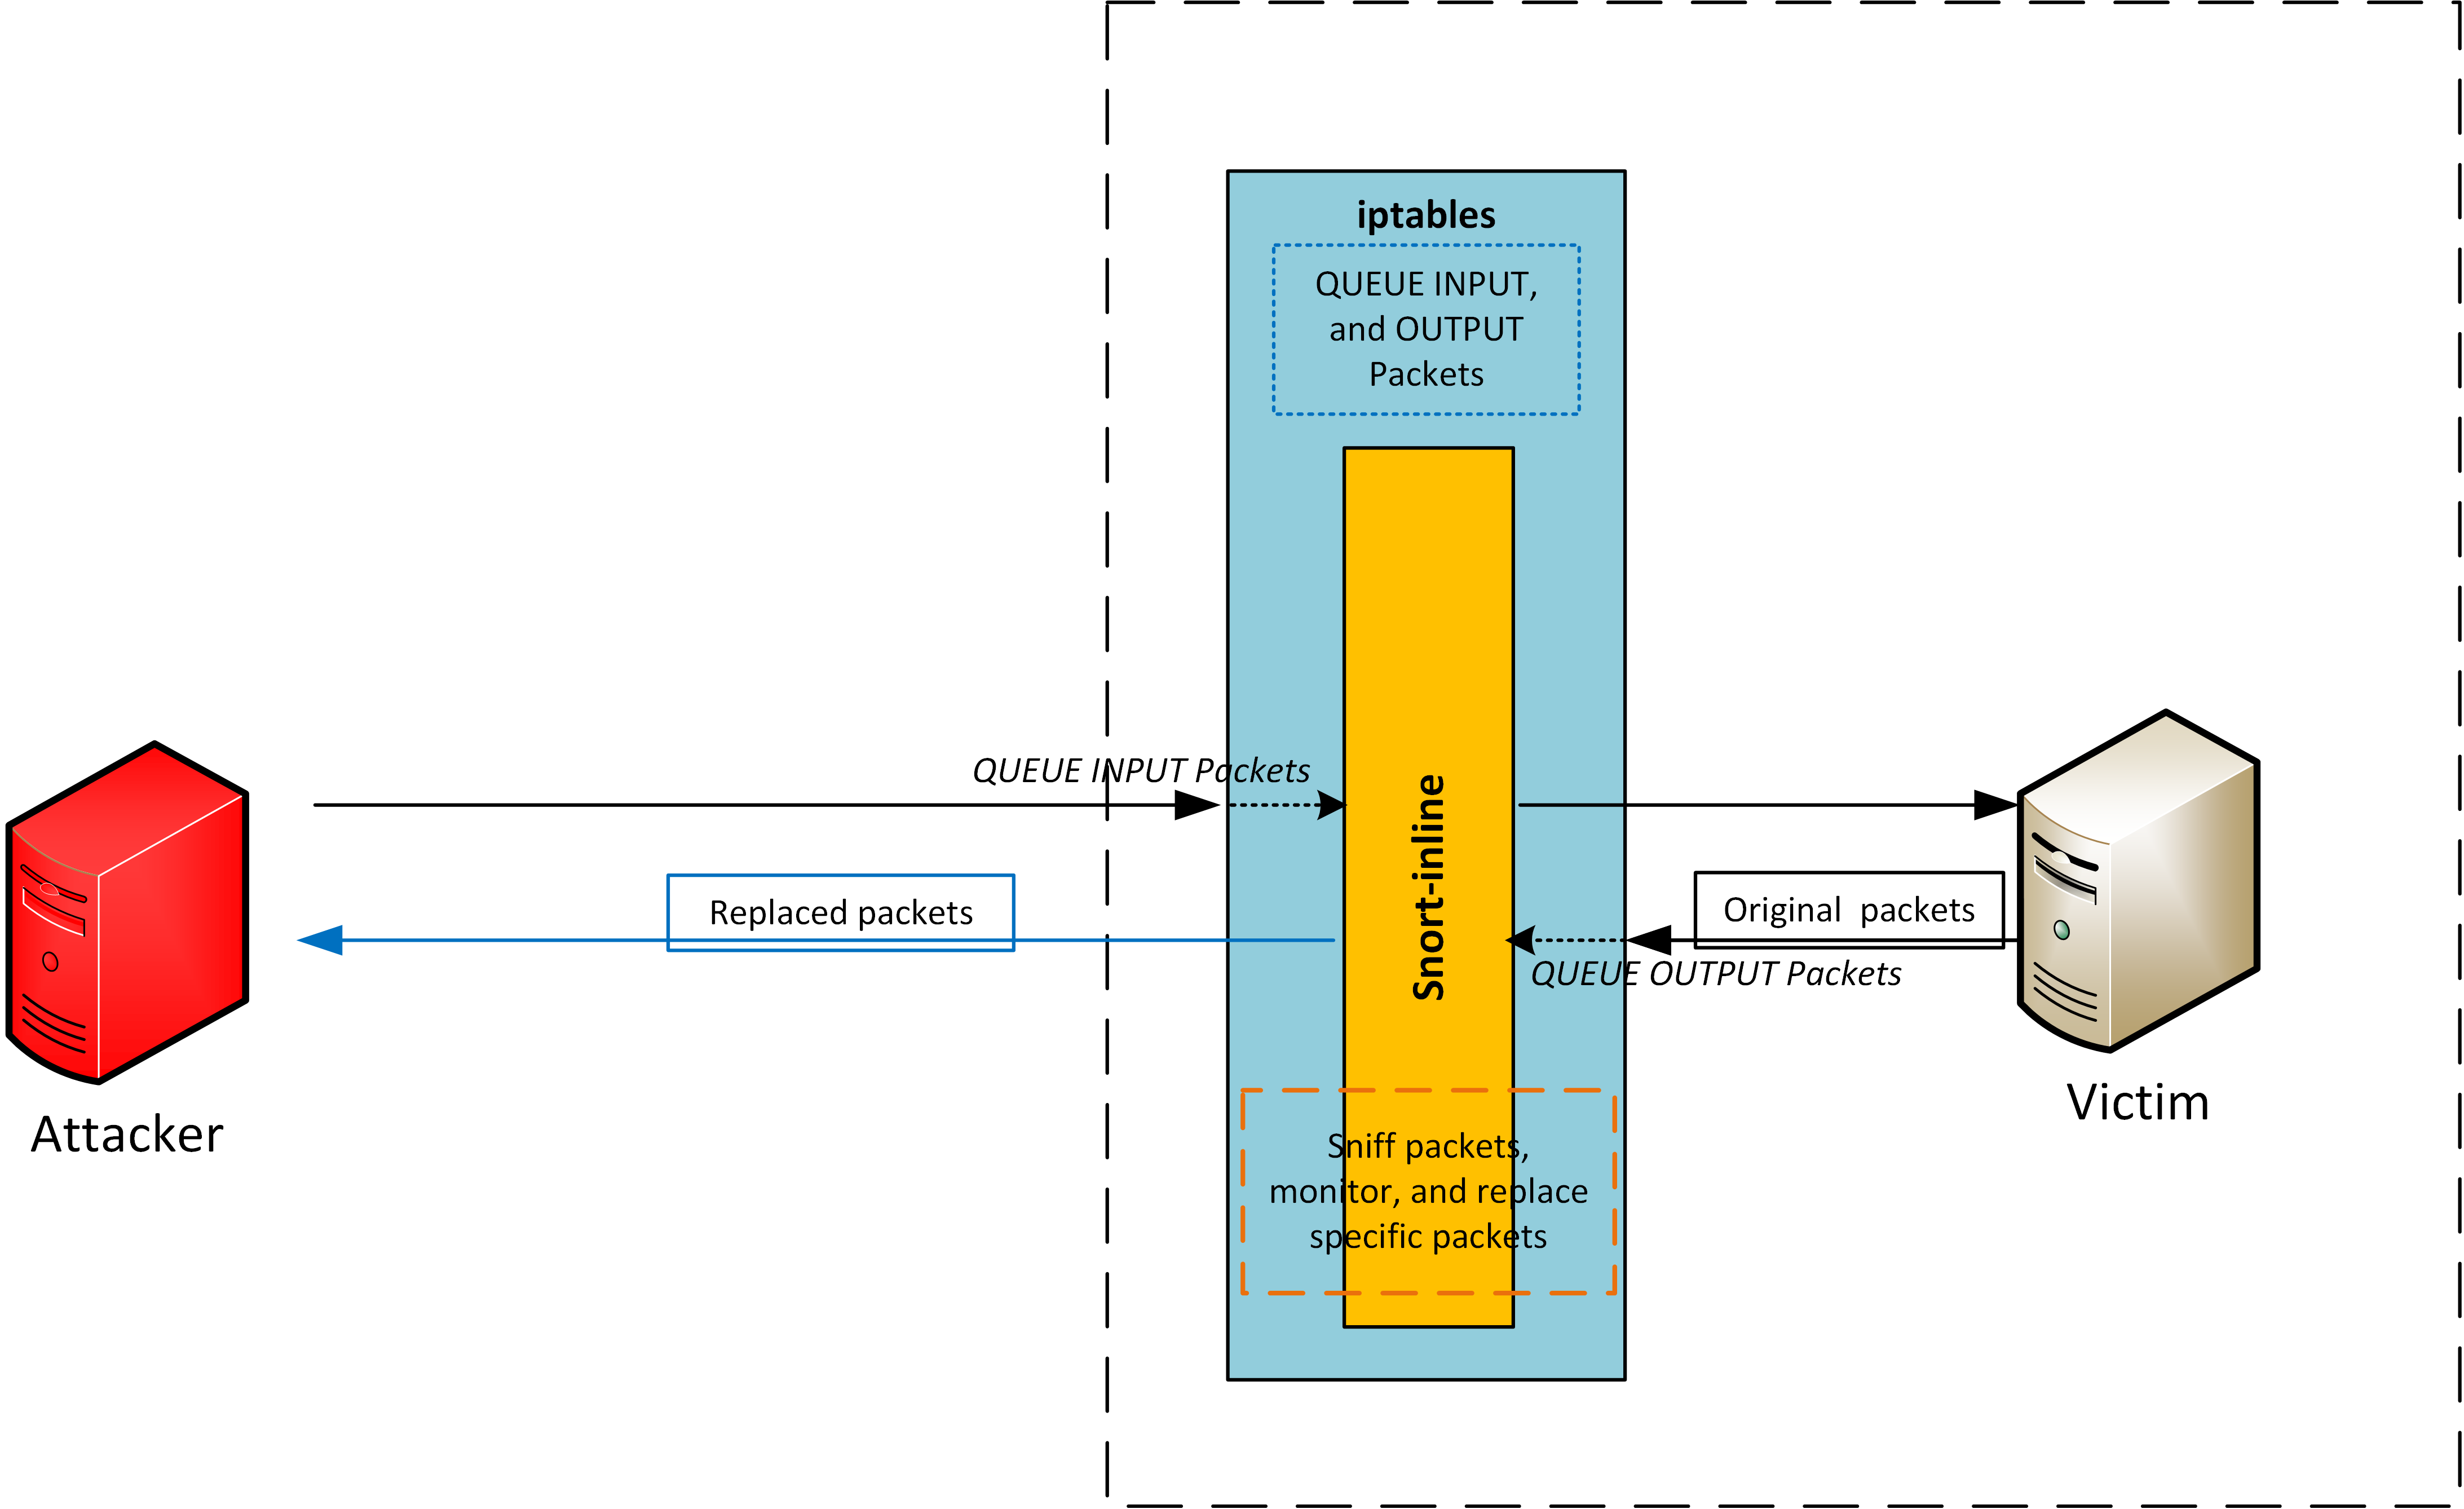
\includegraphics[width=\linewidth]{SnortProcessDiagram_no_back.png}
%\caption{Replacing payload model}
%\label{fig:replacementPayload}
%\end{figure}

%\noindent Figure \ref{fig:replacementPayload} shows how replacing process work on our model. 

In order to forge responses to service fingerprinting attempts, the first step is to queue all the packet not only from the attacker but also all the ingress/egress traffic by iptables. Then, all the traffic will pass through the snort which run as inline mode. The input traffic packets will not be replaced the payload, Snort just only monitor the traffic and try to match with the snort rule. Once the input packets are match with the rule, snort will replace the payload of the original output packet to be pre-payload which is same as vulnerable response. Lastly, the replaced packets that contain a fake response will be sent back to the attacker. Thus, the attacker will learn and get an incorrect information.

\subsection{Overall system setup}

The over-all process of N.A.D.I.R. system is show as Figure \ref{fig:overall}. As development phase of this research, we rebuild whole system by reconfiguring snort and adding snort rules to replace payloads by checking TCP flags of incoming requests \cite{misc:snortflowbit}. We divide snort rules into four different rule files: (1) my-flowbits.rules, (2) my-print.rules, (3) my-snort.rules, and (4) my-drop.rules

The (1) my-flowbits.rules and (2) my-print.rules which we developed at beginning are used to control the process of replacement of any string or payload. The other rule files will maintain by our Java application. At the end we come up with the overall system setup with our java application which takes training label set and once it will regenerate J48 decision tree algorithm by taking unlabeled testing sets or label instead  and it can generate snort rules dynamically. Java application generates snort rules and updates my-snort.rules file as per the training/testing dataset. Java application keep tracking on snort logs and it generates drop rule and update my-drop.rules file if an attack happened and detected. After successfully update snort rules, we managed deamon to restart snort service without missing any packet. We used two different deamon services and created two snort instances and handled two snort instances with two bridge interfaces. Here, if first snort instance is running and once snort rule updated, Java application runs another snort instance with updated rule sets and kill the first snort instance. The system flush entire drop rule file every night and keep the all blacklist IPs into backup file automatically. We tested our model step by step as well in real-time network traffic.


\section{Results}
\label{results}

This section is divided into two parts. In the first, we evaluate the machine learning algorithm and its results for anomaly detection by Intrusion detection system. In the second, we
focus on the overall NADIR system by using Snort to run an experiment in which network attacks are detected and response to with forged honey-service information. NADIR uses the J48 decision tree based learning algorithm to create Snort rules on the fly in response to previously observed network features. An example of a subsection of a classification tree is provided in Figure \ref{fig:J48tree}. Table \ref{table:J48result} and Figure \ref{fig:sum-roc} show the accuracy results of the J48 algorithm and ROC curve for each type of traffic.

\begin{table*}
\begin{center}
\begin{tabular}[width=\textwidth]{llllllllll}
\multicolumn{10}{l}{\bfseries === Detailed Accuracy By Class ===}\\
\\
 & TP Rate & FP Rate & Precision & Recall & F-Measure & MCC & ROC Area & PRC Area & Class\\
 & 0.996 & 0.033 & 0.994 & 0.996 & 0.995 & 0.967 & 0.987 & 0.995 & NORMAL\\
 & 0.976 & 0.003 & 0.981 & 0.976 & 0.979 & 0.975 & 0.991 & 0.977 & Probe\\
 & 0.820 & 0.001 & 0.890 & 0.820 & 0.854 & 0.853 & 0.957 & 0.777 & R2L\\
 & 0.934 & 0.000 & 0.959 & 0.934 & 0.947 & 0.946 & 0.980 & 0.950 & DoS\\
 Weighted Avg. & 0.991 & 0.029 & 0.991 & 0.991 & 0.991 & 0.967 & 0.987 & 0.990 & \\
\end{tabular}
\end{center}
\caption{Accuracy Result of J48 algorithm (based on our dataset)}
\label{table:J48result}
\end{table*}

\begin{figure}[h!]
	\centering
	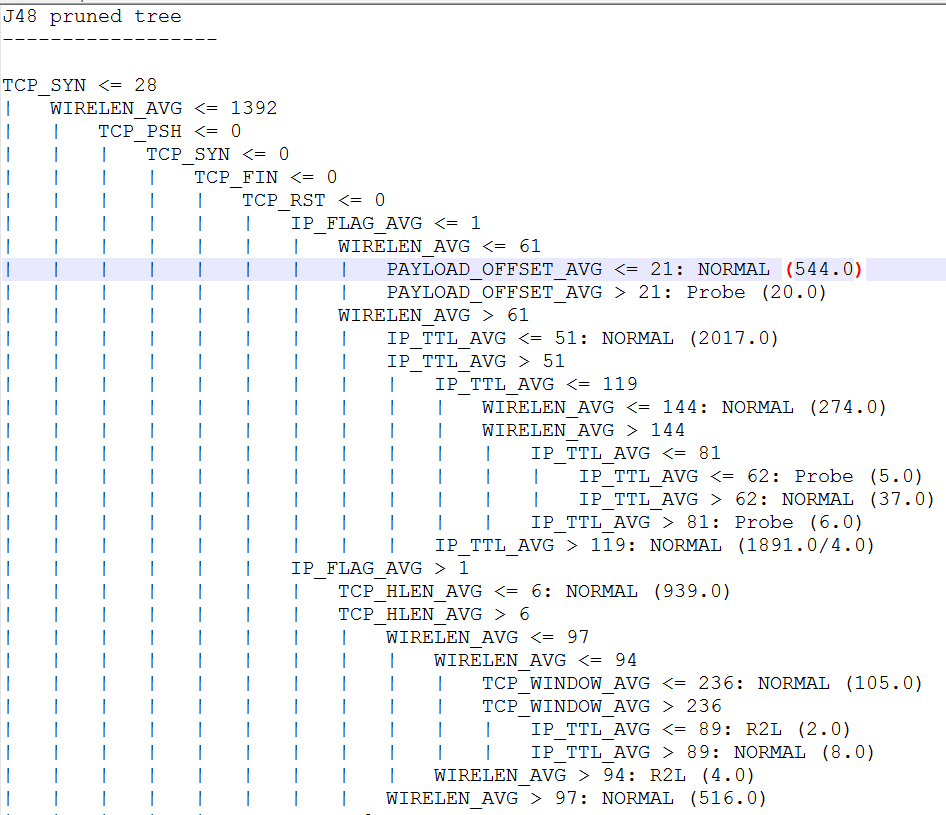
\includegraphics[width=\linewidth]{J48_tree.png}
	\caption{Sub part of pruned tree J48 Decision (based on our dataset)}
	\label{fig:J48tree}
\end{figure}

\begin{figure*}
	\centering
	\begin{subfigure}[t]{0.4\textwidth}
            \centering
            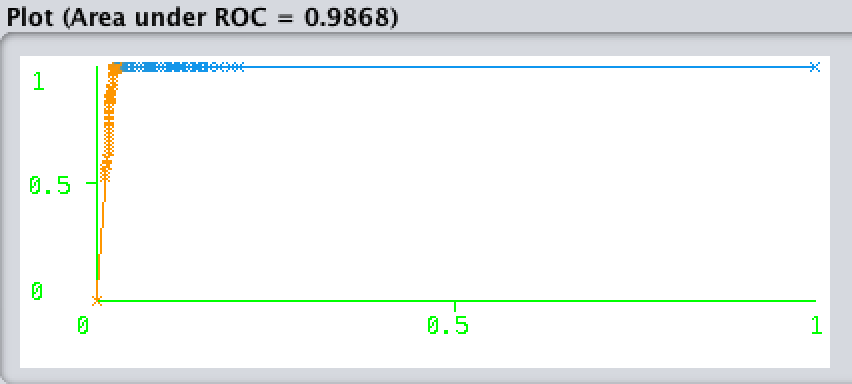
\includegraphics[width=\textwidth]{NORMAL.png}
            \caption{ROC-NORMAL}
            \label{fig:normal-roc}
        \end{subfigure}
        \quad
        \begin{subfigure}[t]{0.4\textwidth}
            \centering
            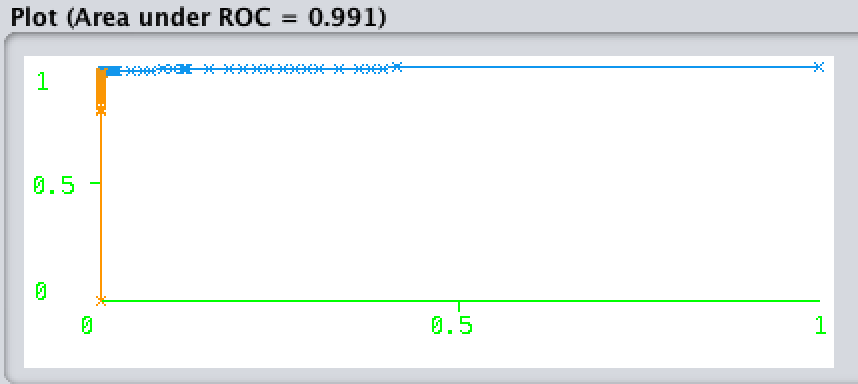
\includegraphics[width=\textwidth]{ProbeAttack.png}
            \caption {ROC-Probe}
            \label{fig:probe-roc}
        \end{subfigure}
        \vskip\baselineskip
        \begin{subfigure}[t]{0.4\textwidth}
            \centering
            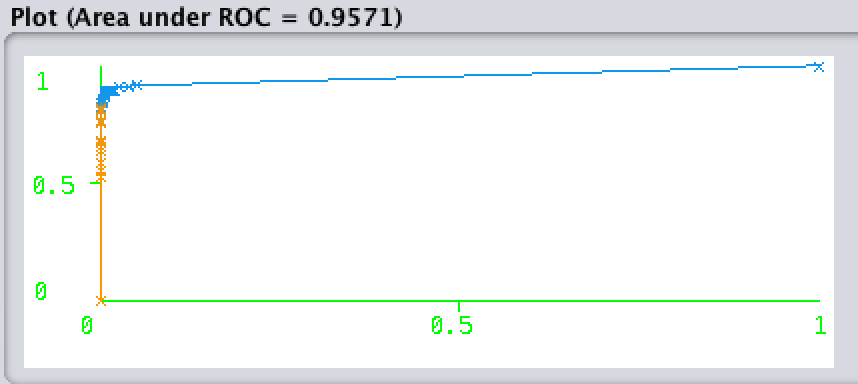
\includegraphics[width=\textwidth]{R2L.png}
            \caption{ROC-R2L}
            \label{fig:r2l-roc}
        \end{subfigure}
        \quad
        \begin{subfigure}[t]{0.4\textwidth}
            \centering
            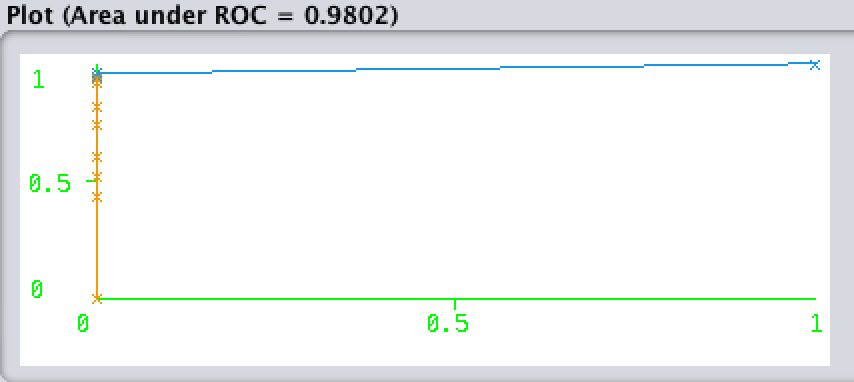
\includegraphics[width=\textwidth]{DoS.png}
            \caption{ROC-DoS}
            \label{fig:dos-roc}
        \end{subfigure}
        \caption{The ROC Curves for each type of traffic}
        \label{fig:sum-roc}
\end{figure*}

We evaluated the end-to-end NADIR system which collects network features, uses them to generate Snort rules, and then pushes them into the configuration of an existing Snort service, which is then 
restarted. This results in an overall system which uses the J48 machine learning algorithm to detect network anomalies. In response, it generates Snort rules dynamically and replaces  them without 
incurring any lost packets. If NADIR detects any attempt to attack the machine, it can respond by taking action such as dropping incoming packets coming from the suspected attacker's IP address.

%We use a common rule for DOS and DDOS detection so machine can detect both of them.

We tested the complete NADIR system by launching attacks against a computer with it installed at known times to provide ground truth. We then calculated area under the ROC curve (AUC) values to evaluate 
the tradeoff between true positive (TP) and false positive (FP) rates of our system. The AUC for detecting these attacks was 0.987 for Normal traffic. NADIR classified Probe, R2L, DoS attacks with AUC 
values of 0.991, 0.950, and 0.980 respectively. Although some errors of both types were made by NADIR's classifier, rates were low; for example, the prediction results of DoS attacks show a 0\% false 
positive rate.


%\section{Discussion}
\label{discussion}

In accuracy results, ROC- space shows area under the curve (AUC) is 98\% of accurate for Normal traffic. It classified Probe, R2L, Dos attacks with 99\%, 95\% and 98\% accurate results respectively. Here, ROC Curves can be used to evaluate the tradeoff between TP (true-positive) and FP (false-positive) rates of classification algorithm. We got some false prediction in which actual attack predicted as normal and same as some normal pattern classified as an attack and got some false alarm by the machine learning classifier. Dos results shows that there is 0.0 FP rate with the classification algorithms.

This study found that the rules of Snort-IDS can be generated and controlled by J48 tree machine learning technique and the feature time-window size (the period of time) of network traffic help us to classify our problem from the higher view because some problems we cannot identify if we analyze the network traffic per packet. We used to work on a unique source IP and destination IP address features, non-duplicate IP Address, per time-window. However, these two features were removed from our feature list in both source and destination because they increase the FP of our result in term of classifying legitimate packets.


\section{Conclusion}
\label{conclusion}

This paper presented NADIR, a system for defending against network reconnaissance efforts. NADIR works by providing deceptive service information when suspicious network contexts are detected. As a part of
this effort we created a tool to generate Snort rules dynamically by observing network traffic in real time. NADIR is capable of hiding information pertaining to real running service and sending back decoy 
information to potential adversaries when suspicious network circumstances are detected. As part of this effort, we collected a network intrusion dataset by observing legitimate traffic on our university 
computer network and injecting real attack data. NADIR is capable of extracting features from observed network packets. As a proof of concept, we implemented NADIR using the J48 decision tree algorithm to 
create an anomaly based IDS, though NADIR is flexible enough to support any approach to intrusion detection. Our experimental results demonstrate that NADIR is capable of providing decoy service information 
as a mitigation strategy to defend against real attacks.

%then generates the Snort rules to detect the malicious pattern. Once Snort-IDS gets the updated rules, application keeps 
%track Snort logs and takes one more forward step to create the drop rules in my-drop.rules to drop network traffic from the specific source IP address which violates the alert rules as it detects threat 
%real-time.

%After we have the final datasets, we use them to feed our NADIR application to generate the dynamic Snort rules. 

%In future work, we will use these techniques to improve the Intrusion Detection System such as identifying dynamically the types of attack in real-time.





% conference papers do not normally have an appendix


% use section* for acknowledgment
%\section*{Acknowledgment}


%The authors would like to thank...





% trigger a \newpage just before the given reference
% number - used to balance the columns on the last page
% adjust value as needed - may need to be readjusted if
% the document is modified later
%\IEEEtriggeratref{8}
% The "triggered" command can be changed if desired:
%\IEEEtriggercmd{\enlargethispage{-5in}}

% references section

% can use a bibliography generated by BibTeX as a .bbl file
% BibTeX documentation can be easily obtained at:
% http://mirror.ctan.org/biblio/bibtex/contrib/doc/
% The IEEEtran BibTeX style support page is at:
% http://www.michaelshell.org/tex/ieeetran/bibtex/
\bibliographystyle{IEEEtran}
% argument is your BibTeX string definitions and bibliography database(s)
%\bibliography{sarnoff_17}
\bibliography{NADIR}
%
% <OR> manually copy in the resultant .bbl file
% set second argument of \begin to the number of references
% (used to reserve space for the reference number labels box)
%\begin{thebibliography}{1}

%\bibitem{IEEEhowto:kopka}
%H.~Kopka and P.~W. Daly, \emph{A Guide to \LaTeX}, 3rd~ed.\hskip 1em plus
%  0.5em minus 0.4em\relax Harlow, England: Addison-Wesley, 1999.

%\end{thebibliography}




% that's all folks
\end{document}
